\newpage
\section{Discussion of Results}
Seismic hazard in northern Iran is computed based on background seismicity and projected on a set of hazard maps. The results obtained are represented as maps for the spatial distribution of horizontal peak ground acceleration with 10\% and 2\% probability of exceedance in 50 years, which correspond to the return period of 475 and 2475 years. The areas of large probabilistic ground motions clearly coincide with zones with a large number of events of magnitude 3.0 and larger. In this study we used two model for seismic hazard calculation, including $M>5$ and $M>4.5$.

\subsection{$\pm$ std}
In this study we use one attenuation relationship (See attenuation relationship section). In order to consider the uncertainty of the ground motion equation we also present the $\pm$ standard deviation of each seismic hazard model. These figures gives an idea about the range of probable peak ground acceleration for 10\% and 2\% probability of exceedance in 50 years. Fig.~\ref{fig:pga_10_minus_plus} and Fig.~\ref{fig:pga_2_minus_plus} show the results of + and - standard deviation of attenuation relationship, respectively.


\begin{figure*} [!ht]
\centering
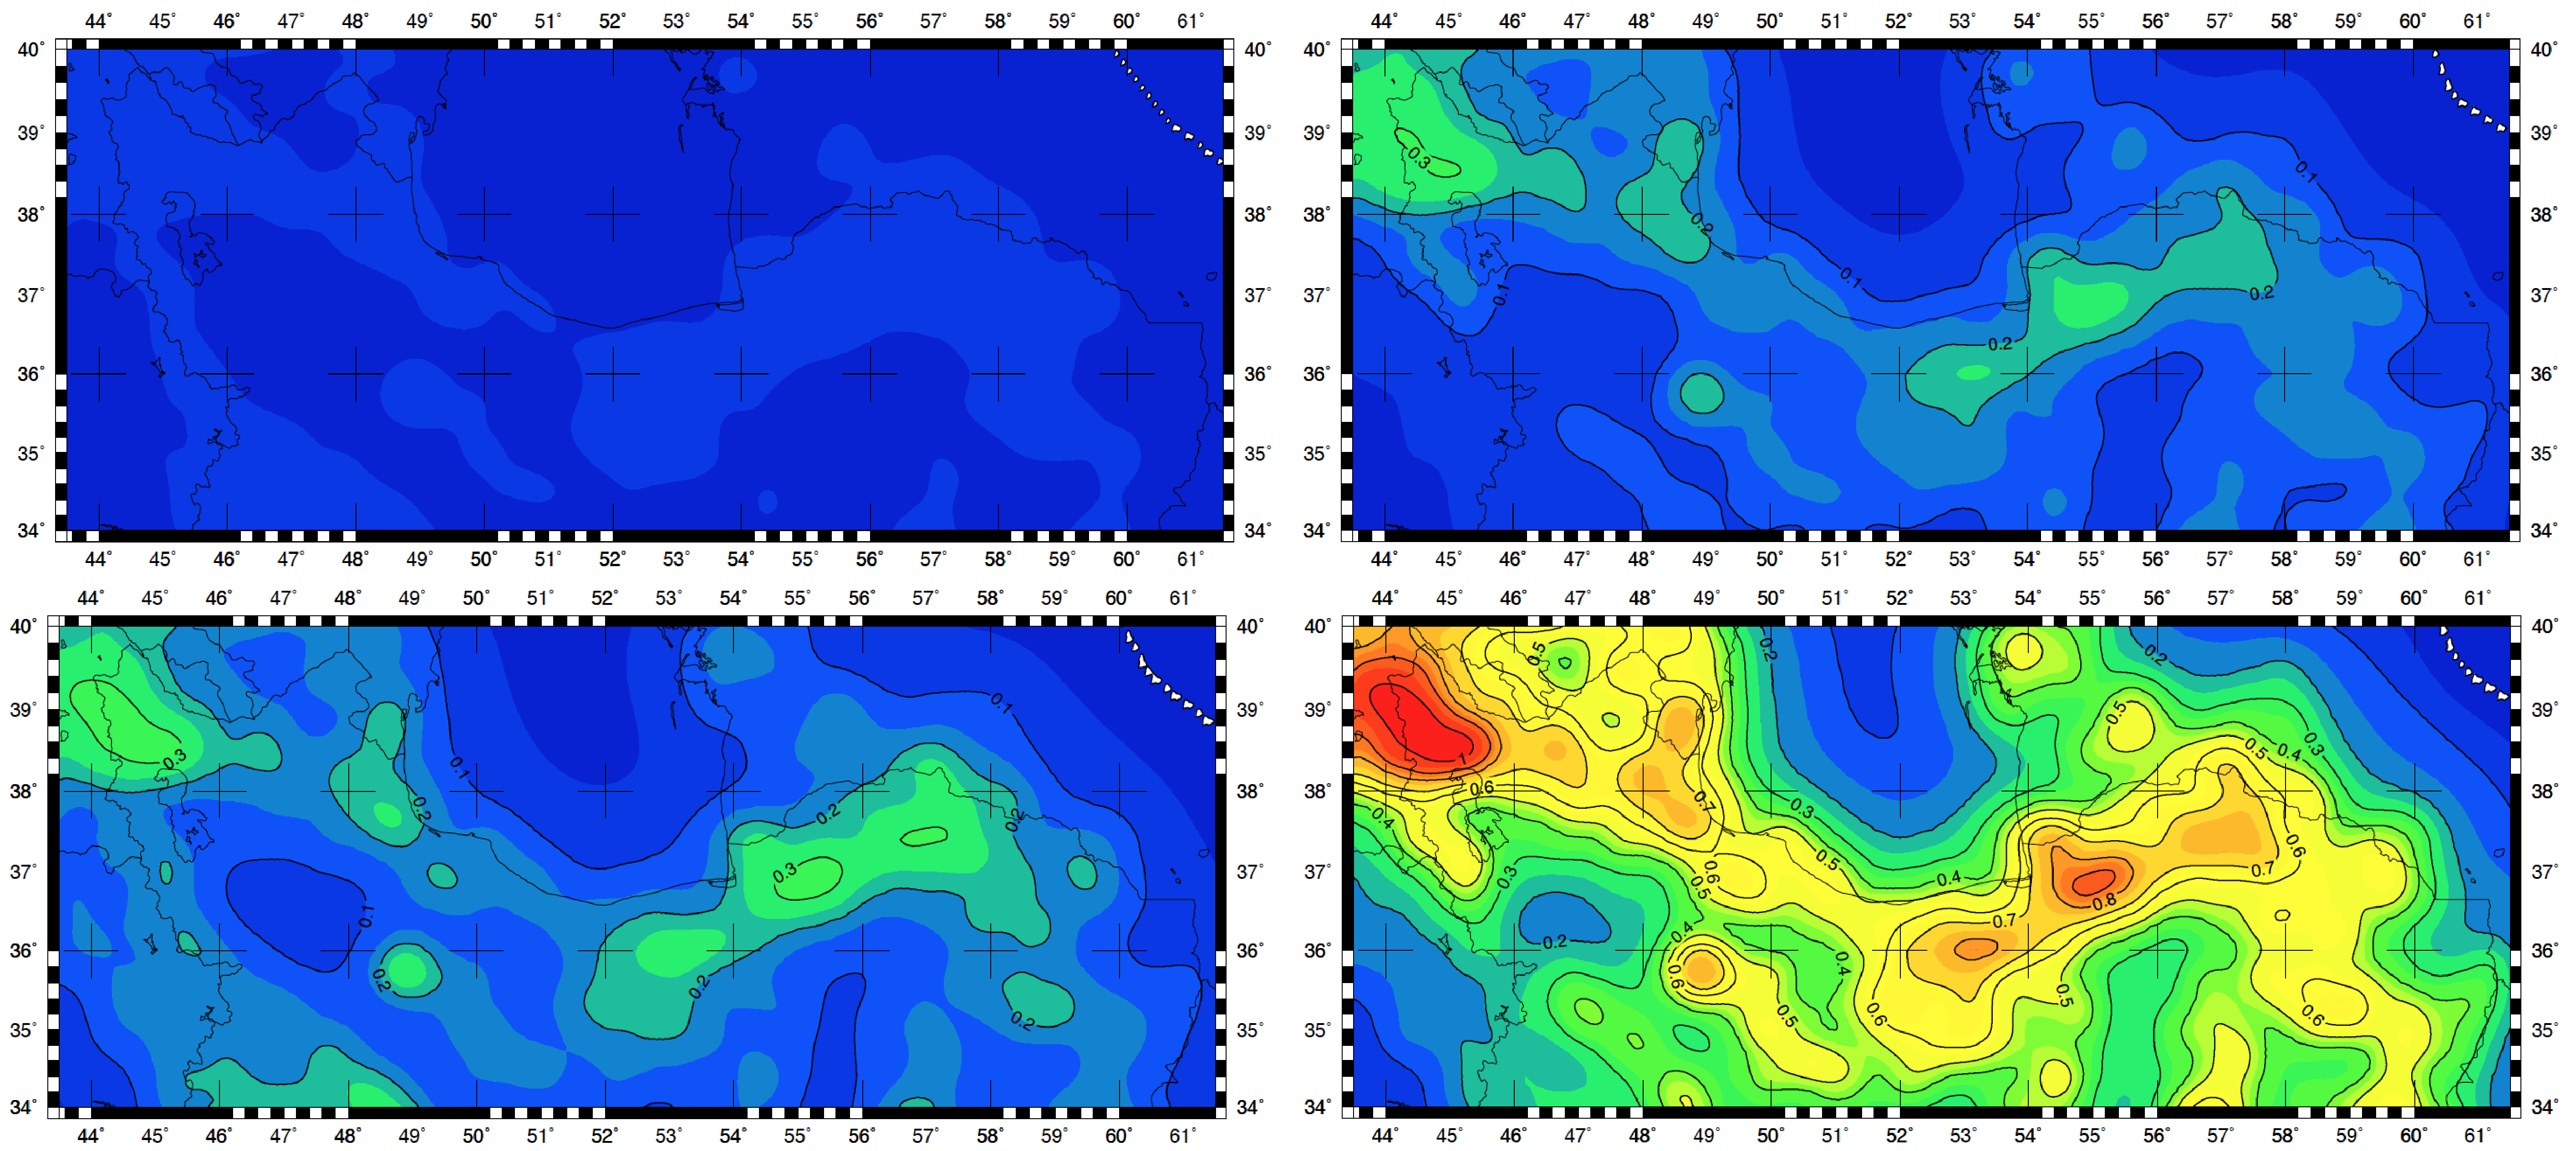
\includegraphics[scale=0.15]{figures/pdf/pga_10_minus_plus.pdf} 
\caption{$\pm$ standard deviation of peak ground acceleration for 10\% probability of exceedance in 50 years.}
\label{fig:pga_10_minus_plus}
\end{figure*}


\begin{figure*} [!ht]
\centering
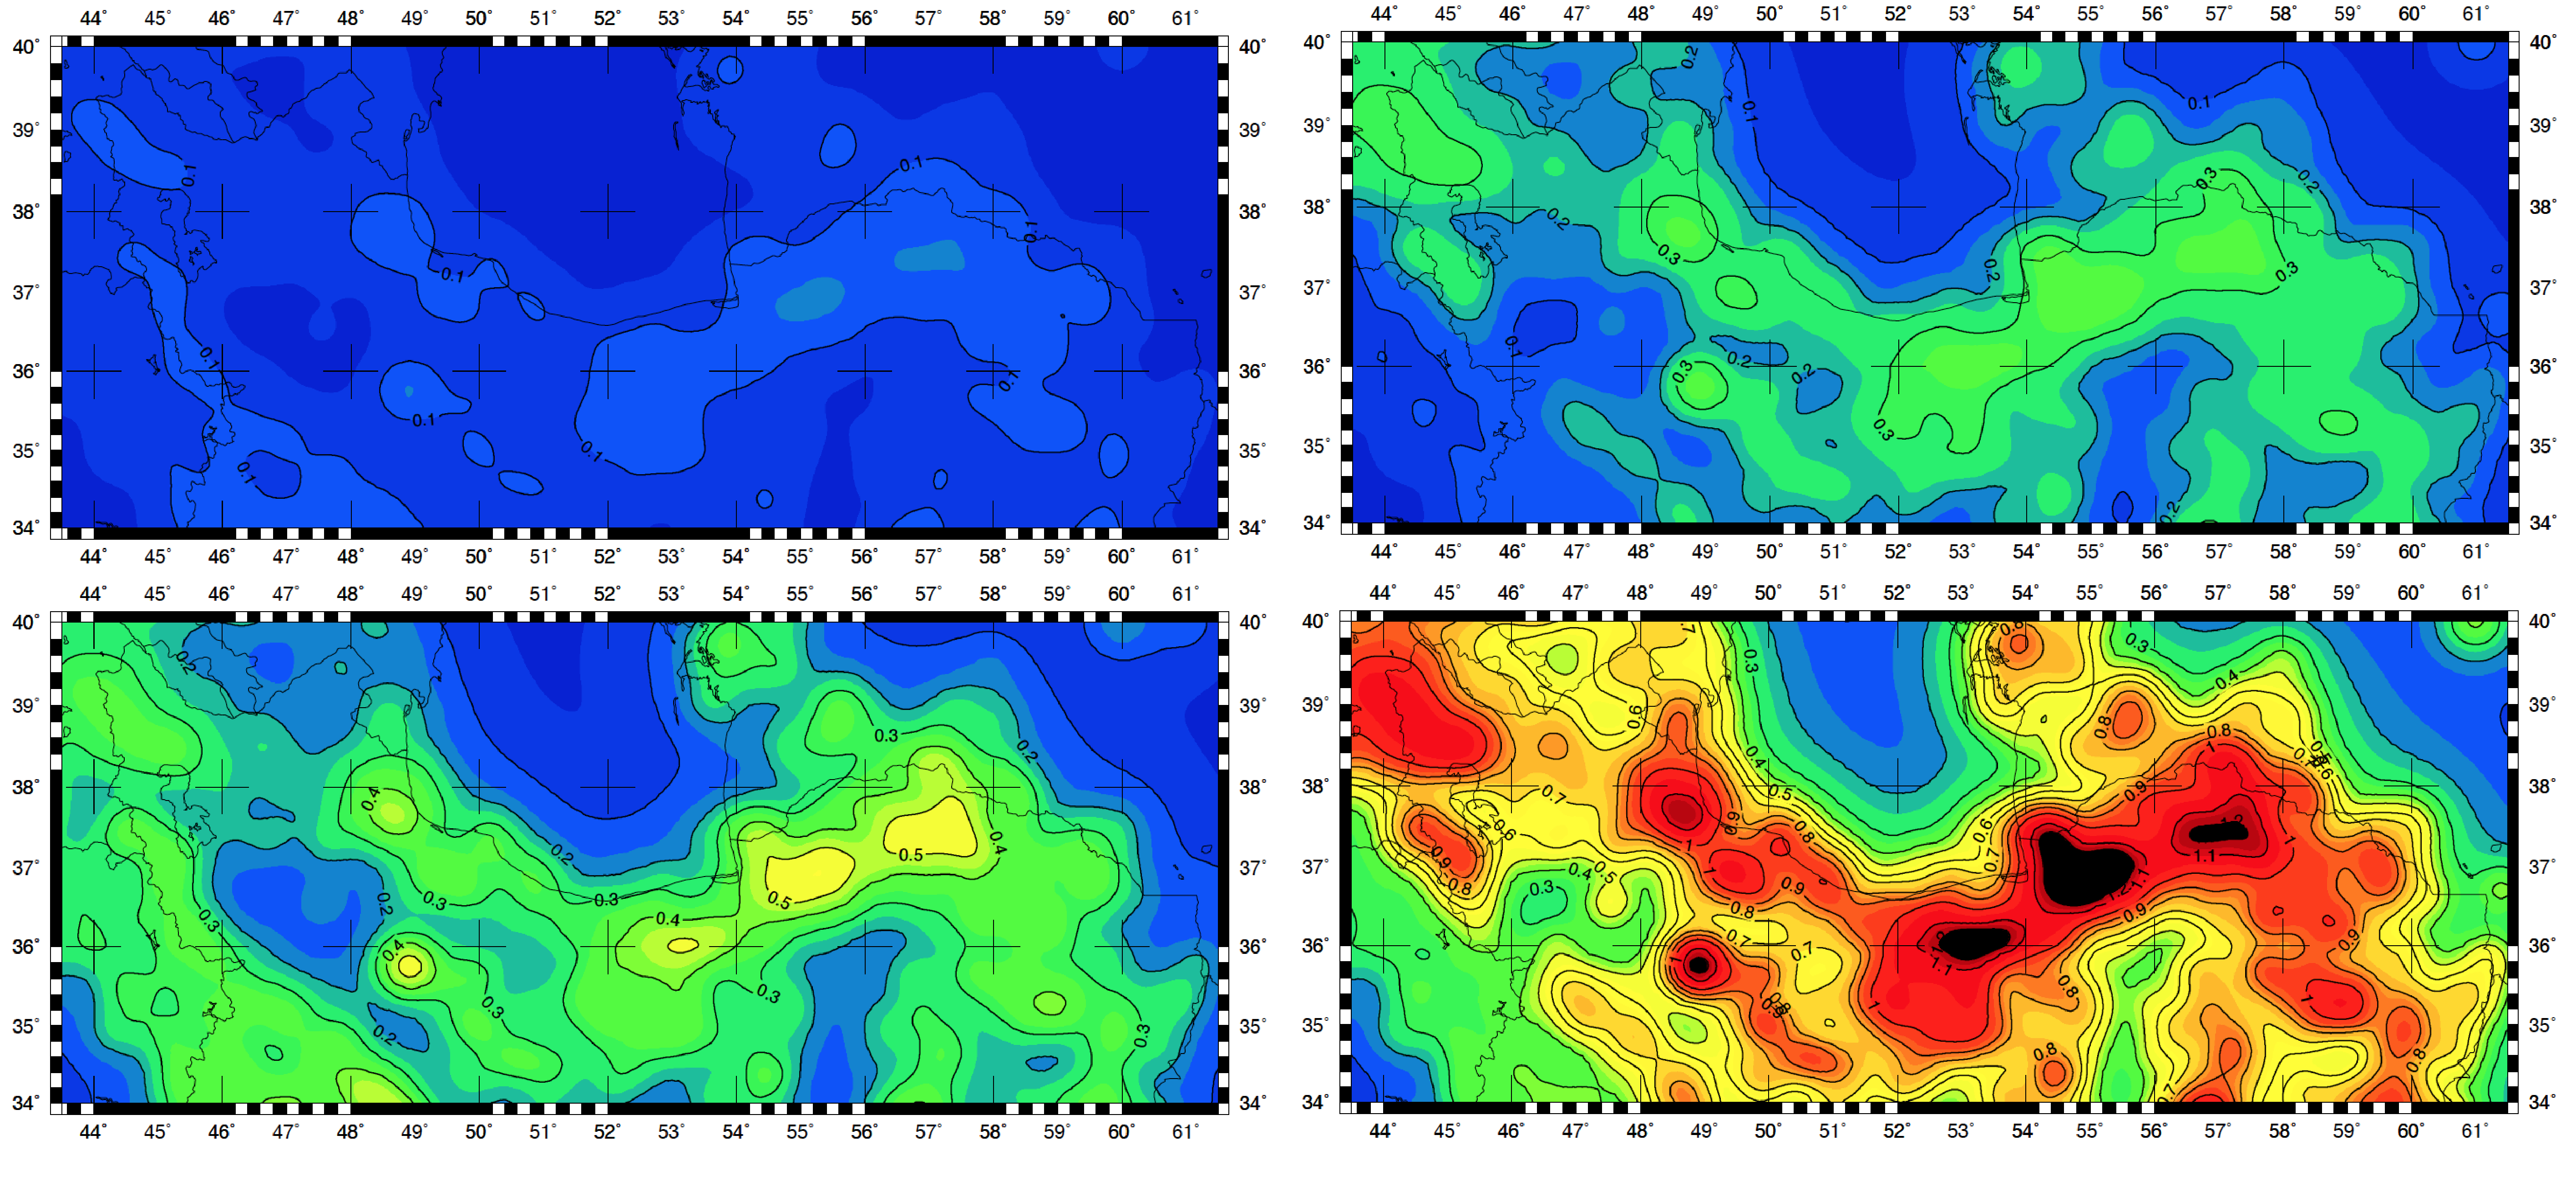
\includegraphics[scale=0.15]{figures/pdf/pga_2_minus_plus.pdf} 
\caption{$\pm$ standard deviation of peak ground acceleration for 2\% probability of exceedance in 50 years.}
\label{fig:pga_2_minus_plus}
\end{figure*}



\subsection{30-70}

\subsection{Hazard Curve}
